\documentclass[fleqn]{article}
\usepackage{amsmath, amssymb, esdiff}
\usepackage{gensymb}
\usepackage{commath}
\usepackage{tikz, pgfplots}
\usepackage{datetime}
\usepackage{ulem}
\usepackage{xcolor}
\usepackage{enumerate}
\setcounter{secnumdepth}{4}
\newcommand\numberthis{\addtocounter{equation}{1}\tag{\theequation}}


%opening
\title{Lecture 5}
\author{Aakash Jog}
\date{\formatdate{11}{11}{2014}}

\begin{document}

\maketitle
%\setlength{\mathindent}{0pt}

\tableofcontents

\newpage
\section{Examples}

\subsection{Example 1}

Two bullets are shot at $t=0$. Their positions, velocities and accelerations are as follows.
\begin{align*}
	\overrightarrow{r_1}(t=0) &= 0 \\
	\overrightarrow{r_2}(t=0) &= 10 \hat{x} \\
	\overrightarrow{v_1} (t=0) &= 50 \hat{x} + 30 \hat{z} \\
	\overrightarrow{v_2} (t=0) &= 40 \hat{y} + 50 \hat{z} \\
	\overrightarrow{a_1} = \overrightarrow{a_2} &= -10 \hat{z} 
\end{align*}

\subsubsection*{Solution}

\begin{align*}
	\overrightarrow{v_1} &= \int \overrightarrow{a_1} \dif t\\
	&= (c_1, c_2, -10 t + c_3)
\end{align*}
\begin{equation*}
	(50, 0, 30) = \overrightarrow{v_1} (t=0) = (c_1, c_2, c_3) 
\end{equation*}
\begin{align*}
	\therefore c_1 &= 50 \\
	\therefore c_2 &= 0 \\
	\therefore c_3 &= 30 \\
	\therefore \overrightarrow{v_1} &= 50 \hat{x} + (30 - 10t) \hat{z}
\end{align*}
\begin{align*}
	\overrightarrow{r_1} &= \int \overrightarrow{v_1}(t) \dif t\\
	&= 50t + d_1 \hat{x} + d_2 \hat{y} + (30t - 5t^2 + d_3) \hat{z}
\end{align*}
\begin{equation*}
(0, 0, 0) = \overrightarrow{r_1} (t=0) = (c_1, c_2, c_3) 
\end{equation*}
\begin{align*}
	\therefore d_1 &= 0 \\
	\therefore d_2 &= 0 \\
	\therefore d_3 &= 0 \\
	\therefore \overrightarrow{r_1} &= 50t \hat{x} + (30t - 5t^2) \hat{z}
\end{align*}
Similarly,
\begin{equation*}
	\overrightarrow{r_2} = 10 \hat{x} + 40 t \hat{y} + (50t - 5t^2) \hat{z}
\end{equation*}
\begin{align*}
	\therefore \overrightarrow{r_{12}} = \overrightarrow{r_2} - \overrightarrow{r_1} &= (10 - 50t , 40t, 20t) \\
	\therefore \left\|\overrightarrow{r_{12}}\right\| &= \sqrt{(10 - 50t)^2 + (40t)^2 + (20t)^2}\\
\end{align*}
Therefore, the velocity of bullet 2 with respect to bullet 1 is
\begin{align*}
	\overrightarrow{v_{2,1}} &= \dod{\overrightarrow{r_{12}}}{t} \\
	&= \dod{\overrightarrow{r_2}}{t} - \dod{\overrightarrow{r_1}}{t} \\
	&= \overrightarrow{v_2} - \overrightarrow{v_1}
\end{align*}

\subsection{Example 2}
Two vehicles, A and B, are moving in space, as given.
\begin{align*}
	\overrightarrow{r_\text{A}} &= (2t + 1) \hat{x} + (2 - 7t) \hat{y} + (3t + 9) \hat{z} \\
	\overrightarrow{r_\text{B}} &= (3t + 2) \hat{x} + (4t - 5) \hat{y} + (t + 1) \hat{z} \\
	\overrightarrow{v_\text{A}} &= (2, -7, 3) \\
	\overrightarrow{v_\text{B}} &= (3, 4, 1)
\end{align*}
Find the angle between the velocities of A and B.\\
Find the velocity of A with respect to B. \\
At $t=0$, a package is thrown from vehicle A, and it reaches vehicle B at $t=5$. What is the velocity of the package with respect to vehicle A?
\subsubsection*{Solution}

\begin{align*}
	\cos \theta &= \dfrac{\overrightarrow{v_\text{A}} \cdot \overrightarrow{v_\text{B}}}{v_\text{A} v_\text{B}} \\
	\overrightarrow{v_{\text{A,B}}} &= \overrightarrow{v_\text{A}} - \overrightarrow{v_\text{B}} \\
	&= (-1, -11, 2)
\end{align*}
The motion of the package can be represented by 
\begin{align*}
	r_\text{P} &= r_\text{B} (t=5) - r_\text{A}(t=0)\\
	&= (16, 13, -3)\\
	\therefore \overrightarrow{v_\text{P}} &= \dfrac{1}{5} (16, 13, -3)\\
	\therefore \overrightarrow{v_\text{P,A}} &= \overrightarrow{v_P} - \overrightarrow{v_A}\\
	&= \left( \dfrac{16}{5} - 2 , \dfrac{13}{5} - (-7), \dfrac{-3}{5} - 3 \right) \\
	&= \left(\dfrac{6}{5} , \dfrac{48}{5}, \dfrac{12}{5}\right)
\end{align*}

\section{General Non-linear Motion}

\begin{align*}
\overrightarrow{r} &= r \hat{r} \\
\overrightarrow{v} = \dot{\overrightarrow{r}} &= \dot{r} \hat{r} + r \dot{\theta} \hat{\theta} \\
\overrightarrow{a} = \ddot{\overrightarrow{r}} &= \left(\ddot{r} - r(\dot{\theta})^2\right) \hat{r} + \left(2 \dot{r} \dot{\theta} + r \ddot{\theta}\right) \hat{\theta}
\end{align*}

\begin{tikzpicture}
\draw [<->] (0,-4) -- (0,4);
\draw [<->] (-4,0) -- (4,0); 

\draw [->] (0,0) -- (35:4) node [midway, below right] {$\hat{r}(t)$};
\draw [->] (0,0) -- (40:4) node [midway, above left] {$\hat{r}(t + \dif t)$};
\draw [->, red] (35:4) -- (40:4) node [midway, above right] {$\dif \hat{r}$};

\draw [->] (0,0) -- (125:4) node [midway, above right] {$\hat{\theta}(t)$};
\draw [->] (0,0) -- (130:4) node [midway, below left] {$\hat{\theta}(t + \dif t)$};
\draw [->, red] (125:4) -- (130:4) node [midway, above left] {$\dif \hat{\theta}$};
\end{tikzpicture}

\section{Circular Motion}

Circular motion is a special case of of non-linear motion with $\dot{r} = 0$.

\begin{equation*}
	\dod{\hat{r}}{t} = \dfrac{\hat{r}(t + \dif t) - \hat{r}(t)}{\dif t}
\end{equation*}

\begin{align*}
	r &= R = \text{constant} \\
	\dot{r} &= \ddot{r} = 0 \\
	\omega &\doteq \dot{\theta} = \text{angular velocity} \\
	\alpha &\doteq \ddot{\theta} = \text{angular acceleration}\\
	\overrightarrow{v} &= R \dot{\theta} \hat{\theta} \\
	&= R \omega \hat{\theta} \\
	\overrightarrow{a} &= - R (\dot{\theta})^2 \hat{r} + R \ddot{\theta} \hat{\theta} \\
	&= -R \omega^2 \hat{r} + R \alpha \hat{\theta}
\end{align*}

\begin{tikzpicture}
	\draw [<->] (-5,0) -- (5,0);
	\draw [<->] (0,-5) -- (0,5);
	
	\draw (0,0) circle [radius=4];
	
	\fill (35:4) circle [radius=2pt];
	
	\draw [->] (0,0) -- (35:4) node [midway, above] {$R$}; 
	\draw [green, ->] (0,0) -- (35:1) node [above] {$\hat{r}$};
	\draw [green, ->] (0,0) -- (125:1) node [above] {$\hat{\theta}$};
	\draw [green, ->] (35:4) -- (35:3) node [below] {$\overrightarrow{a}$};
	\draw [red, ->] (35:4) -- ++(125:2) node [above] {$\hat{v}$};
\end{tikzpicture}

\subsection{Circular Motion With Constant Angular Velocity}

\begin{align*}
	v &= \omega R \hat{\theta}\\
	a &= - \omega^2 R \hat{r} 
\end{align*}

\subsection{Examples}

\subsubsection{Example 1}

\begin{tikzpicture}
	\draw (0,4) arc [radius = 4, start angle=90, end angle=180];
	\draw [dashed] (0,0) -- (0,4);
	\draw [dashed] (0,0) -- (-4,0) node [below, midway] {$R$};
	
	\fill (145:4) circle [radius=2pt];
	
	\draw [->] (145:4) -- ++(55:2) node [left] {$v$};
	\draw [->] (145:4) -- ++(-35:2) node [below] {$f$};
\end{tikzpicture}\\
The friction responsible for the centripetal force is static friction. This can be evident as it can change to various values to accommodate different velocities. Kinetic friction will not exhibit such a behaviour.
\begin{align*}
	f_s &= m \dfrac{v^2}{R} \\
	&\leq \mu_s N = \mu_s m g \\
	\therefore m \dfrac{v^2}{R} &\leq \mu_s m g\\
	\therefore v^2 &\leq \mu_s R g \\
	\therefore v &\leq \sqrt{\mu_s R g} 
\end{align*}

\subsubsection{Banked Roads}

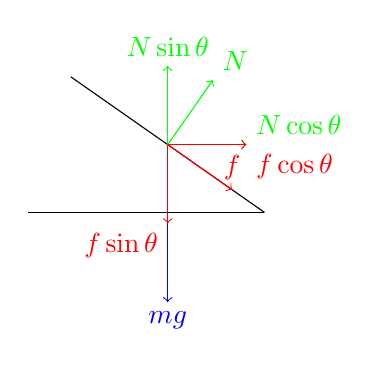
\begin{tikzpicture}
	\draw (0,0) -- (145:3);
	\draw (0,0) -- (-3,0);
	
	\draw [green, ->] (145:1.5) -- ++(55:1) node [above right ] {$N$};
	\draw [green, ->] (145:1.5) -- ++(90:1) node [above] {$N \sin \theta$};
	\draw [green, ->] (145:1.5) -- ++(0:1) node [above right] {$N \cos \theta$};
	
	\draw [blue, ->] (145:1.5) -- ++(-90:2) node [below] {$mg$};

	\draw [red, ->] (145:1.5) -- ++(-35:1) node [above] {$f$};
	\draw [red, ->] (145:1.5) -- ++(0:1) node [below right] {$f \cos \theta$};
	\draw [red, ->] (145:1.5) -- ++(-90:1) node [below left] {$f \sin \theta$};
\end{tikzpicture}\\
If $v = \sqrt{g R \tan \theta}$
\begin{equation*}
	f = 0
\end{equation*}
If $v > \sqrt{g R \tan \theta}$
\begin{equation*}
	N \sin \theta + f \cos \theta = m \dfrac{v^2}{R}
\end{equation*}
The velocity can be increased till $f$ reaches its maximum, i.e. $f = \mu_s N$.
\begin{align*}
	N \sin \theta + \mu_s N \cos \theta &= m \dfrac{v^2}{R} \\
	mg + \mu_s N \sin \theta &= N \cos \theta \\
	\therefore N \cos \theta - \mu_s N \sin \theta &= mg
\end{align*}
\begin{equation*}
	\therefore v_{\text{max}} = \sqrt{g R \dfrac{\sin \theta + \mu_s \cos \theta}{\cos \theta - \mu_s \sin \theta}}
\end{equation*}
If $v > \sqrt{g R \tan \theta}$, the friction in in the opposite direction.
\begin{equation*}
\therefore v_{\text{min}} = \sqrt{g R \dfrac{\sin \theta - \mu_s \cos \theta}{\cos \theta + \mu_s \sin \theta}}
\end{equation*}
\end{document}